\chapter{Cas du triangle}
\label{Cas du Triangle}

\section{Algorithme d'obtention de la solution optimale}
\label{Algo optimal cas triangulaire}

Règles permettant de trouver le premier mouvement d'une solution optimale
\begin{easylist}[articletoc]
& Toutes les stations sont équilibrées.
&& \underline{$p \ne q$}

   Aller de $p$ à $q$.
&& \underline{$p = q$}

   Ne pas bouger (c'est fini).
& Il existe une station non-équlibrée.
&& \underline{$p$ est équilibrée ou en défaut.}

    Aller sur une station en excès sans emporter de vélos.
&& \underline{$p$ est en excès}
&&& \underline{$x(p)-y(p) \ge C$.}

    Prendre C vélos et les déposer sur une station en défaut différente de $q$ s'il en existe, sur $q$ sinon.
&&& \underline{$x(p)-y(p) < C$.}

    Prendre $x(p)-y(p)$ vélos.
&&&& \underline{Les deux autres stations sont en défaut.}

     Déposer les vélos pris sur une station différente de $q$.
&&&& \underline{Une seule autre station est en défaut.}

     On note $r$ la troisième station en excès ou équilibrée\\
     et $\cE = x(r) - y(r) \pmod{C}$ avec $1 \le \cE \le C$.
&&&&& \underline{$x(p)-y(p)+\cE > C$.}

      Aller sur la station en défaut et déposer les vélos.

&&&&& \underline{$x(p)-y(p)+\cE \le C$.}

      Aller sur la station en excès et déposer les vélos.
\end{easylist}

\section{Optimalité de l'algorithme précédent}

\begin{figure}[ht]
  \label{Notation graphe triangulaire}
  \center 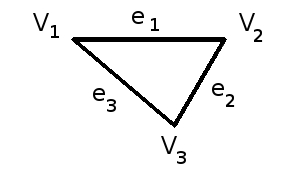
\includegraphics[scale=0.5]{graphe_triangulaire_notations.jpg}
  \caption{Notations utilisées dans le cas du graphe triangulaire}
\end{figure}

Le changement de variables décrit en section \ref{Changement variables} s'écrit ici :
\begin{equation}\notag
  \left\{
    \begin{aligned}
      \zeta_1 &= z_1 + z_3 \\
      \zeta_2 &= z_1 + z_2 \\
      \zeta_3 &= z_2 + z_3
    \end{aligned}
  \right.
  \quad \mbox{et} \quad
  \left(
    \begin{array}{c}
      z_1 \\
      z_2 \\
      z_3
    \end{array}
  \right)
  = \frac{1}{2}
  \left(
    \begin{array}{rrr}
      1 & 1 & -1 \\
      -1 & 1 & 1 \\
      1 & -1 & 1
    \end{array}
  \right)
  \left(
    \begin{array}{c}
      \zeta_1 \\
      \zeta_2 \\
      \zeta_3
    \end{array}
  \right)
\end{equation}
En remplaçant dans la fonction objectif, on obtient :
\begin{equation}\notag
  \sum_{i=1}^3c_iz_i =
    \frac{1}{2} \displayUB{ \left(c_1 - c_2 + c_3 \right) }{>0} \zeta_1
  + \frac{1}{2} \displayUB{ \left(c_1 + c_2 - c_3 \right) }{>0} \zeta_2
  + \frac{1}{2} \displayUB{ \left(-c_1 + c_2 + c_3\right) }{>0} \zeta_3 >0
\end{equation}
Les coefficients des $\zeta_i$ sont positifs à cause de l'hytohèse d'inégalité triangulaire évoquée en section \ref{sec: Inégalité triangulaire}.
\\

Pour un sommet $v \in V$, on définit $U_v$ par $\{v\}$ si $v$ est en excès ou équilibré et par $\overline{\{v\}}$ sinon. On définit également
\[
\zeta_v(p,q,\bs{x},\bs{y}) = \mbox{max} \left( 2 \left\lceil \frac{x(U_v)-y(U_v)}{C} \right\rceil\ + \eta(p,q,U_v), \mu(p,q,U_v,\bs{x},\bs{y}) \right)
\]

\begin{thm}\label{Optimalite algo graphe triangulaire}
\emph{Optimalité de l'algorithme \ref{Algo optimal cas triangulaire}}

L'algorithme précédent donne le premier mouvement d'une solution optimale et le coût de cette solution est donnée par
\[
\frac{1}{2} \left(c_1 - c_2 + c_3 \right) \zeta_1(p,q,\bs{x},\bs{y})
+ \frac{1}{2} \left(c_1 + c_2 - c_3 \right) \zeta_2(p,q,\bs{x},\bs{y})
+ \frac{1}{2} \left(-c_1 + c_2 + c_3\right) \zeta_3(p,q,\bs{x},\bs{y}).
\]
\end{thm}

\section{Preuve de l'optimalité de l'algorithme}

Les coefficients des $\zeta_v$ étant positifs, il suffit de montrer que les $\zeta_v$ atteignent leur borne inférieure pour montrer que l'on a minimisé le coût de la solution. Si l'on montre que pour tout sommet $v \in V$, on a $\zeta_v = \zeta_v(p,q,\bs{x},\bs{y})$ à chaque étape de l'algorithme, alors, par défnition de $\zeta_v(p,q,\bs{x},\bs{y})$,  $\zeta_v$ sera bien égal à sa borne inférieure.

Il suffit donc de montrer l'égalité suivante pour tout $v \in V$
\begin{gather} \label{Récurrence triangle}
  \zeta_v(p,q,\bs{x},\bs{y}) = \left\{
  \begin{array}{ll}
    1+\zeta_v(p',q,\bs{x'},\bs{y}) & \mbox{si } v=p \mbox{ ou } v=p' \\
    \zeta_v(p',q,\bs{x'},\bs{y}) & \mbox{sinon}
  \end{array}
  \right.
\end{gather}
Nous allons effectuer cette démonstration par récurrence sur les mouvements du camion.
\\

Dans chacun des différents cas, l'égalité \eqref{Récurrence triangle} est évidente si $v \ne p$ et $v \ne p'$.

\subsection*{Cas 1.1 et 1.2}

L'égalité \eqref{Récurrence triangle} est évidente dans ce cas.

\subsection*{Cas 2.1}

\begin{minipage}{0.5\linewidth}
\begin{itemize}
\item $p$ équilibrée ou en défaut
\item $p'$ en excès
\item on ne transporte pas de vélos
\end{itemize}
\end{minipage}
\begin{minipage}{0.5\linewidth}
\begin{center}
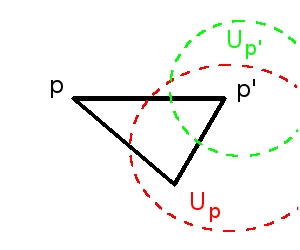
\includegraphics[scale=0.5]{graphe_triangulaire_21.jpg}
\end{center}
\end{minipage}

On note $A = 2 \left\lceil \frac{\displaystyle x(U_p)-y(U_p)}{\displaystyle C} \right\rceil$

\begin{gather*}
  \begin{array}{r|c|c|c|c||c|}
    \multicolumn{2}{c|}{}
    & 2 \left\lceil \frac{x(U_p)-y(U_p)}{C} \right\rceil
    & \eta(p,q,U_p)
    & \mu(p,q,U_p,\bs{x},\bs{y})
    & \zeta_p(p,q,\bs{x},\bs{y})
    \\ \hline
    \multirow{2}{*}{$p$ équilibrée}
    & p=q
    & \multirow{2}{*}{= A = 0}
    & 0
    & 2
    & 2
    \\ \cdashline{2-2}\cdashline{4-6}
    & p \ne q
    &
    & 1
    & 1
    & 1
    \\ \hline
    \multirow{2}{*}{$p$ en défaut}
    & p=q
    & \multirow{2}{*}{$= A \ge 2$}
    & 0
    & 2
    & A
    \\ \cdashline{2-2}\cdashline{4-6}
    & p \ne q
    &
    & 1
    & 1
    & A + 1
    \\ \hline
  \end{array}
\end{gather*}

\begin{gather*}
  \begin{array}{r|c|c|c|c||c|}
    \multicolumn{2}{c|}{}
    & 2 \left\lceil \frac{x'(U_p)-y(U_p)}{C} \right\rceil
    & \eta(p',q,U_p)
    & \mu(p',q,U_p,\bs{x'},\bs{y})
    & \zeta_p(p',q,\bs{x'},\bs{y})
    \\ \hline
    \multirow{2}{*}{$p$ équilibrée}
    & p=q
    & \multirow{2}{*}{= A = 0}
    & -1
    & 1
    & 1
    \\ \cdashline{2-2}\cdashline{4-6}
    & p \ne q
    &
    & 0
    & 0
    & 0
    \\ \hline
    \multirow{2}{*}{$p$ en défaut}
    & p=q
    & \multirow{2}{*}{$= A \ge 2$}
    & -1
    & 1
    & A-1
    \\ \cdashline{2-2}\cdashline{4-6}
    & p \ne q
    &
    & 0
    & 2
    & A
    \\ \hline
  \end{array}
\end{gather*}
Donc $\zeta_p(p,q,\bs{x},\bs{y}) = 1 + \zeta_p(p',q,\bs{x'},\bs{y})$.
\\

On note $B = 2 \left\lceil \frac{\displaystyle x(U_{p'})-y(U_{p'})}{\displaystyle C} \right\rceil$.

\begin{gather*}
  \begin{array}{r|c|c|c||c|}
    & 2 \left\lceil \frac{x(U_{p'})-y(U_{p'})}{C} \right\rceil
    & \eta(p,q,U_{p'})
    & \mu(p,q,U_{p'},\bs{x},\bs{y})
    & \zeta_{p'}(p,q,\bs{x},\bs{y})
    \\ \hline
    p' = q
    & \multirow{2}{*}{$= B \ge 2$}
    & 1
    & 1
    & B + 1
    \\ \cline{1-1}\cline{3-5}
    p' \ne q
    &
    & 0
    & 2
    & B
    \\ \hline
  \end{array}
\end{gather*}

\begin{gather*}
  \begin{array}{r|c|c|c||c|}
    & 2 \left\lceil \frac{x'(U_{p'})-y(U_{p'})}{C} \right\rceil
    & \eta(p',q,U_{p'})
    & \mu(p',q,U_{p'},\bs{x'},\bs{y})
    & \zeta_{p'}(p',q,\bs{x'},\bs{y})
    \\ \hline
    p' = q
    & \multirow{2}{*}{$= B \ge 2$}
    & 0
    & 2
    & B
    \\ \cline{1-1}\cline{3-5}
    p' \ne q
    &
    & -1
    & 1
    & B - 1
    \\ \hline
  \end{array}
\end{gather*}
Donc $\zeta_{p'}(p,q,\bs{x},\bs{y}) = 1 + \zeta_{p'}(p',q,\bs{x'},\bs{y})$.

\subsection*{Cas 2.2.1}

\begin{minipage}{0.5\linewidth}
\begin{itemize}
\item $p$ en excès
\item $p'$ en défaut
\item on transporte $C$ vélos
\item $x(p)-y(p) \ge C$
\end{itemize}
\end{minipage}
\begin{minipage}{0.5\linewidth}
\begin{center}
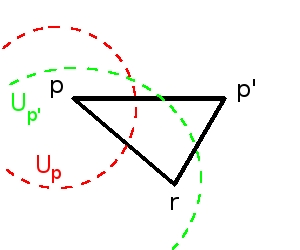
\includegraphics[scale=0.5]{graphe_triangulaire_221.jpg}
\end{center}
\end{minipage}

On note $A = 2 \left\lceil \frac{\displaystyle x(U_p)-y(U_p)}{\displaystyle C} \right\rceil$.

\begin{gather*}
  \begin{array}{c|c|c|c|c||c|}
    \multicolumn{2}{c|}{}
    & 2 \left\lceil \frac{x(U_p)-y(U_p)}{C} \right\rceil
    & \eta(p,q,U_p)
    & \mu(p,q,U_p,\bs{x},\bs{y})
    & \zeta_p(p,q,\bs{x},\bs{y})
    \\ \hline
    p \mbox{ équilibrée}
    & p=q
    & \multirow{2}{*}{$2$}
    & 0
    & 2
    & 2
    \\ \cdashline{2-2}\cdashline{4-6}
    \mbox{après mouvement}
    & p \ne q
    &
    & -1
    & 1
    & 1
    \\ \hline
    p \mbox{ en excès}
    & p=q
    & \multirow{2}{*}{$= A \ge 4$}
    & 0
    & 2
    & A
    \\ \cdashline{2-2}\cdashline{4-6}
    \mbox{après mouvement}
    & p \ne q
    &
    & -1
    & 1
    & A-1
    \\ \hline
  \end{array}
\end{gather*}

\begin{gather*}
  \begin{array}{c|c|c|c|c||c|}
    \multicolumn{2}{c|}{}
    & 2 \left\lceil \frac{x'(U_p)-y(U_p)}{C} \right\rceil
    & \eta(p',q,U_p)
    & \mu(p',q,U_p,\bs{x'},\bs{y})
    & \zeta_p(p',q,\bs{x'},\bs{y})
    \\ \hline
    p \mbox{ équilibrée}
    & p=q
    & \multirow{2}{*}{$0$}
    & 1
    & 1
    & 1
    \\ \cdashline{2-2}\cdashline{4-6}
    \mbox{après mouvement}
    & p \ne q
    &
    & 0
    & 0
    & 0
    \\ \hline
    p \mbox{ en excès}
    & p=q
    & \multirow{2}{*}{$= A-2 \ge 2$}
    & 1
    & 1
    & A-1
    \\ \cdashline{2-2}\cdashline{4-6}
    \mbox{après mouvement}
    & p \ne q
    &
    & 0
    & 2
    & A-2
    \\ \hline
  \end{array}
\end{gather*}
Donc $\zeta_p(p,q,\bs{x},\bs{y}) = 1 + \zeta_p(p',q,\bs{x'},\bs{y})$.
\\

On note $B = 2 \left\lceil \frac{\displaystyle x(U_{p'})-y(U_{p'})}{\displaystyle C} \right\rceil$.

\begin{gather*}
  \begin{array}{r|c|c|c||c|}
    & 2 \left\lceil \frac{x(U_{p'})-y(U_{p'})}{C} \right\rceil
    & \eta(p,q,U_{p'})
    & \mu(p,q,U_{p'},\bs{x},\bs{y})
    & \zeta_{p'}(p,q,\bs{x},\bs{y})
    \\ \hline
    p' = q
    & \multirow{2}{*}{$= B \ge 2$}
    & -1
    & 1
    & B - 1
    \\ \cline{1-1}\cline{3-5}
    p' \ne q
    &
    & 0
    & 2
    & B
    \\ \hline
  \end{array}
\end{gather*}

\underline{$1^{er}$ sous-cas : $p'$ reste en défaut après le mouvement}
\begin{gather*}
  \begin{array}{r|c|c|c||c|}
    & 2 \left\lceil \frac{x'(U_{p'})-y(U_{p'})}{C} \right\rceil
    & \eta(p',q,U_{p'})
    & \mu(p',q,U_{p'},\bs{x'},\bs{y})
    & \zeta_{p'}(p',q,\bs{x'},\bs{y})
    \\ \hline
    p' = q
    & \multirow{2}{*}{$= B-2 \ge 2$}
    & 0
    & 2
    & B-2
    \\ \cline{1-1}\cline{3-5}
    p' \ne q
    &
    & 1
    & 1
    & B - 1
    \\ \hline
  \end{array}
\end{gather*}

\underline{$2^{ème}$ sous-cas : $p'$ est équlibrée ou en excès après le mouvement}\\
On se place après le mouvement de $p$ à $p'$.
\begin{itemize}
\item \underline{Si $p'=q$}, alors comme $p$ est équilibrée ou en excès, on en déduit que $r$ est équilibrée ou en défaut.\\
Or $r$ n'est pas en défaut (sinon, on serait aller sur $r$ car $p'=q$). Donc $r$ est équilibrée.\\
On en déduit que $p$ et $p'$ sont également équilibrées.\\
D'où : $\zeta_{p'}(p,q,\bs{x},\bs{y}) = 1$ et $\zeta_{p'}(p',q,\bs{x'},\bs{y}) = 0$.

\item \underline{Si $p' \ne q$}
\begin{equation}\notag
\zeta_{p'}(p,q,\bs{x},\bs{y})
= \mbox{max} \left( 2 \left\lceil \frac{x(U_{p'})-y(U_{p'})}{C} \right\rceil + 0, 2\right)
= 2 \left\lceil \frac{ x(U_{p'})-y(U_{p'})}{C} \right\rceil
\end{equation}
\begin{equation}\notag
\zeta_{p'}(p',q,\bs{x'},\bs{y})
= \mbox{max} \left( 2 \left\lceil \frac{x'(U_{p'})-y(U_{p'})}{C} \right\rceil + 1, 1\right)
= 2 \left\lceil \frac{x(U_{p'})-y(U_{p'})}{C} \right\rceil - 1
\end{equation}
\end{itemize}
Dans les deux cas, $\zeta_{p'}(p,q,\bs{x},\bs{y}) = 1 + \zeta_{p'}(p',q,\bs{x'},\bs{y})$.

\subsection*{Cas 2.2.2.1}

\begin{minipage}{0.5\linewidth}
\begin{itemize}
\item $p$ en excès
\item $p'$ et $r$ en défaut
\item $p' \ne q$
\item on transporte $x(p)-y(p)$ vélos
\item $x(p)-y(p) < C$
\end{itemize}
\end{minipage}
\begin{minipage}{0.5\linewidth}
\begin{center}
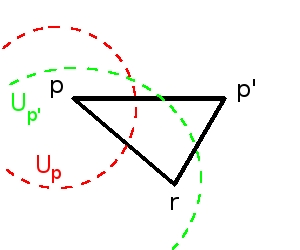
\includegraphics[scale=0.5]{graphe_triangulaire_221.jpg}
\end{center}
\end{minipage}

\begin{gather*}
  \begin{array}{c|c|c|c||c|}
    & 2 \left\lceil \frac{x(U_p)-y(U_p)}{C} \right\rceil
    & \eta(p,q,U_p)
    & \mu(p,q,U_p,\bs{x},\bs{y})
    & \zeta_p(p,q,\bs{x},\bs{y})
    \\ \hline
    p=q
    & \multirow{2}{*}{$2$}
    & 0
    & 2
    & 2
    \\ \cline{1-1}\cline{3-5}
    p \ne q
    &
    & -1
    & 1
    & 1
    \\ \hline
  \end{array}
\end{gather*}

\begin{gather*}
  \begin{array}{c|c|c|c||c|}
    & 2 \left\lceil \frac{x'(U_p)-y(U_p)}{C} \right\rceil
    & \eta(p',q,U_p)
    & \mu(p',q,U_p,\bs{x'},\bs{y})
    & \zeta_p(p',q,\bs{x'},\bs{y})
    \\ \hline
    p=q
    & \multirow{2}{*}{$0$}
    & 1
    & 1
    & 1
    \\ \cline{1-1}\cline{3-5}
    p \ne q
    &
    & 0
    & 0
    & 0
    \\ \hline
  \end{array}
\end{gather*}
Donc $\zeta_p(p,q,\bs{x},\bs{y}) = 1 + \zeta_p(p',q,\bs{x'},\bs{y})$.
\\

\[\zeta_{p'}(p,q,\bs{x},\bs{y}) = \mbox{max}\left(2 \left\lceil \frac{x(U_{p'})-y(U_{p'})}{C} \right\rceil + 0, 2\right)\]
Or $x(U_{p'})-y(U_{p'})<C$ (sinon, $r$ serait en excès).
Donc $\zeta_{p'}(p,q,\bs{x},\bs{y}) = 2$.

\[\zeta_{p'}(p',q,\bs{x'},\bs{y}) = \mbox{max}\left(2 \left\lceil \frac{x'(U_{p'})-y(U_{p'})}{C} \right\rceil + 1,1\right)\]
Or $x(U_{p'})-y(U_{p'})<0$ (car $p$ est équilibrée et $r$ est en défaut).
Donc $\zeta_{p'}(p',q,\bs{x'},\bs{y}) = 1$.
\\
\\
Donc $\zeta_{p'}(p,q,\bs{x},\bs{y}) = 1 + \zeta_{p'}(p',q,\bs{x'},\bs{y})$.

\subsection*{Cas 2.2.2.2.1}

\begin{minipage}{0.5\linewidth}
\begin{itemize}
\item $p$ en excès
\item $p'$ en défaut
\item $r$ en excès ou équilibrée
\item on transporte $x(p)-y(p)$ vélos
\item $x(p)-y(p) < C$
\item $x(p) - y(p) + \cE > C$
\end{itemize}
\end{minipage}
\begin{minipage}{0.5\linewidth}
\begin{center}
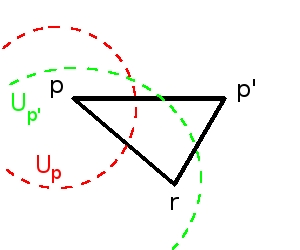
\includegraphics[scale=0.5]{graphe_triangulaire_221.jpg}
\end{center}
\end{minipage}

\begin{gather*}
  \begin{array}{c|c|c|c||c|}
    & 2 \left\lceil \frac{x(U_p)-y(U_p)}{C} \right\rceil
    & \eta(p,q,U_p)
    & \mu(p,q,U_p,\bs{x},\bs{y})
    & \zeta_p(p,q,\bs{x},\bs{y})
    \\ \hline
    p=q
    & \multirow{2}{*}{$2$}
    & 0
    & 2
    & 2
    \\ \cline{1-1}\cline{3-5}
    p \ne q
    &
    & -1
    & 1
    & 1
    \\ \hline
  \end{array}
\end{gather*}

\begin{gather*}
  \begin{array}{c|c|c|c||c|}
    & 2 \left\lceil \frac{x'(U_p)-y(U_p)}{C} \right\rceil
    & \eta(p',q,U_p)
    & \mu(p',q,U_p,\bs{x'},\bs{y})
    & \zeta_p(p',q,\bs{x'},\bs{y})
    \\ \hline
    p=q
    & \multirow{2}{*}{$0$}
    & 1
    & 1
    & 1
    \\ \cline{1-1}\cline{3-5}
    p \ne q
    &
    & 0
    & 0
    & 0
    \\ \hline
  \end{array}
\end{gather*}
Donc $\zeta_p(p,q,\bs{x},\bs{y}) = 1 + \zeta_p(p',q,\bs{x'},\bs{y})$.
\\

On note $\gamma \in \NN \cup \{-1\}$ l'entier tel que $x(r)-y(r)=\gamma C + \cE$. Alors :
\[
2 \left\lceil \frac{x(U_{p'})-y(U_{p'})}{C} \right\rceil
= 2 \left\lceil \frac{x(p)-y(p)+x(r)-y(r)}{C} \right\rceil
= 2 \left\lceil \frac{x(p)-y(p)+\gamma C + \cE}{C} \right\rceil
= 2\gamma + 4
\]
\[
2 \left\lceil \frac{x'(U_{p'})-y(U_{p'})}{C} \right\rceil
= 2 \left\lceil \frac{x'(p)-y(p)+x'(r)-y(r)}{C} \right\rceil
= 2 \left\lceil \frac{x(r)-y(r)}{C} \right\rceil
= 2 \left\lceil \frac{\gamma C + \cE}{C} \right\rceil
= 2\gamma + 2
\]
De plus, $\gamma = -1$ si et seulement si $r$ est équilibrée.

\begin{gather*}
  \begin{array}{c|c|c|c|c||c|}
    \multicolumn{2}{c|}{}
    & 2 \left\lceil \frac{x(U_{p'})-y(U_{p'})}{C} \right\rceil
    & \eta(p,q,U_{p'})
    & \mu(p,q,U_{p'},\bs{x},\bs{y})
    & \zeta_{p'}(p,q,\bs{x},\bs{y})
    \\ \hline
    \multirow{2}{*}{$r$ équilibrée}
    & p'=q
    & \multirow{2}{*}{$2\gamma+4=2$}
    & -1
    & 1
    & 1
    \\ \cdashline{2-2}\cdashline{4-6}
    & p' \ne q
    &
    & 0
    & 2
    & 2
    \\ \hline
    \multirow{2}{*}{$r$ en excès}
    & p'=q
    & \multirow{2}{*}{$2\gamma+4 \ge 4$}
    & -1
    & 1
    & 2\gamma+3
    \\ \cdashline{2-2}\cdashline{4-6}
    & p' \ne q
    &
    & 0
    & 2
    & 2\gamma+4
    \\ \hline
  \end{array}
\end{gather*}

\begin{gather*}
  \begin{array}{c|c|c|c|c||c|}
    \multicolumn{2}{c|}{}
    & 2 \left\lceil \frac{x'(U_{p'})-y(U_{p'})}{C} \right\rceil
    & \eta(p',q,U_{p'})
    & \mu(p',q,U_{p'},\bs{x'},\bs{y})
    & \zeta_{p'}(p',q,\bs{x'},\bs{y})
    \\ \hline
    \multirow{2}{*}{$r$ équilibrée}
    & p'=q
    & \multirow{2}{*}{$2\gamma+2=0$}
    & 0
    & 0
    & 0
    \\ \cdashline{2-2}\cdashline{4-6}
    & p' \ne q
    &
    & 1
    & 1
    & 1
    \\ \hline
    \multirow{2}{*}{$r$ en excès}
    & p'=q
    & \multirow{2}{*}{$2\gamma+2 \ge 2$}
    & 0
    & 2
    & 2\gamma+2
    \\ \cdashline{2-2}\cdashline{4-6}
    & p' \ne q
    &
    & 1
    & 1
    & 2\gamma+3
    \\ \hline
  \end{array}
\end{gather*}
Donc $\zeta_{p'}(p,q,\bs{x},\bs{y}) = 1 + \zeta_{p'}(p',q,\bs{x'},\bs{y})$.

\subsection*{Cas 2.2.2.2.2}

\begin{minipage}{0.5\linewidth}
\begin{itemize}
\item $p$ en excès
\item $p'=r$ en excès
\item la troisième station est en défaut
\item on transporte $x(p)-y(p)$ vélos
\item $x(p)-y(p) < C$
\item $x(p) - y(p) + \cE \le C$
\end{itemize}
\end{minipage}
\begin{minipage}{0.5\linewidth}
\begin{center}
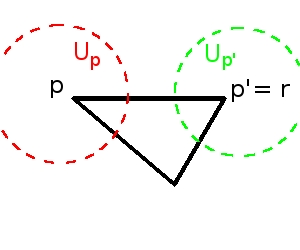
\includegraphics[scale=0.5]{graphe_triangulaire_22222.jpg}
\end{center}
\end{minipage}

\begin{gather*}
  \begin{array}{c|c|c|c||c|}
    & 2 \left\lceil \frac{x(U_p)-y(U_p)}{C} \right\rceil
    & \eta(p,q,U_p)
    & \mu(p,q,U_p,\bs{x},\bs{y})
    & \zeta_p(p,q,\bs{x},\bs{y})
    \\ \hline
    p=q
    & \multirow{2}{*}{$2$}
    & 0
    & 2
    & 2
    \\ \cline{1-1}\cline{3-5}
    p \ne q
    &
    & -1
    & 1
    & 1
    \\ \hline
  \end{array}
\end{gather*}

\begin{gather*}
  \begin{array}{c|c|c|c||c|}
    & 2 \left\lceil \frac{x'(U_p)-y(U_p)}{C} \right\rceil
    & \eta(p',q,U_p)
    & \mu(p',q,U_p,\bs{x'},\bs{y})
    & \zeta_p(p',q,\bs{x'},\bs{y})
    \\ \hline
    p=q
    & \multirow{2}{*}{$0$}
    & 1
    & 1
    & 1
    \\ \cline{1-1}\cline{3-5}
    p \ne q
    &
    & 0
    & 0
    & 0
    \\ \hline
  \end{array}
\end{gather*}
Donc $\zeta_p(p,q,\bs{x},\bs{y}) = 1 + \zeta_p(p',q,\bs{x'},\bs{y})$.
\\

On note $\gamma \in \NN \cup \{-1\}$ l'entier tel que $x(p')-y(p') = x(r)-y(r) = \gamma C + \cE$. Alors :
\[
2 \left\lceil \frac{x(U_{p'})-y(U_{p'})}{C} \right\rceil
= 2 \left\lceil \frac{x(p')-y(p')}{C} \right\rceil
= 2 \left\lceil \frac{\gamma C + \cE}{C} \right\rceil
= 2\gamma + 2
\]
\[
2 \left\lceil \frac{x'(U_{p'})-y(U_{p'})}{C} \right\rceil
= 2 \left\lceil \frac{x'(p')-y(p')}{C} \right\rceil
= 2 \left\lceil \frac{x(p)-y(p)+\gamma C + \cE}{C} \right\rceil
= 2\gamma + 2
\]
De plus, si $\gamma = -1$, alors $p'$ est équilibrée ou en défaut, ce qui est faux. Donc $\gamma \ge 0$

\begin{gather*}
  \begin{array}{c|c|c|c||c|}
    & 2 \left\lceil \frac{x(U_{p'})-y(U_{p'})}{C} \right\rceil
    & \eta(p,q,U_{p'})
    & \mu(p,q,U_{p'},\bs{x},\bs{y})
    & \zeta_{p'}(p,q,\bs{x},\bs{y})
    \\ \hline
    p'=q
    & \multirow{2}{*}{$2 \gamma + 2 \ge 2$}
    & 1
    & 1
    & 2 \gamma + 3
    \\ \cline{1-1}\cline{3-5}
    p' \ne q
    &
    & 0
    & 2
    & 2\gamma + 2
    \\ \hline
  \end{array}
\end{gather*}

\begin{gather*}
  \begin{array}{c|c|c|c||c|}
    & 2 \left\lceil \frac{x'(U_{p'})-y(U_{p'})}{C} \right\rceil
    & \eta(p',q,U_{p'})
    & \mu(p',q,U_{p'},\bs{x'},\bs{y})
    & \zeta_{p'}(p',q,\bs{x'},\bs{y})
    \\ \hline
    p'=q
    & \multirow{2}{*}{$2 \gamma + 2 \ge 2$}
    & 0
    & 2
    & 2 \gamma + 2
    \\ \cline{1-1}\cline{3-5}
    p' \ne q
    &
    & -1
    & 1
    & 2\gamma + 1
    \\ \hline
  \end{array}
\end{gather*}
Donc $\zeta_{p'}(p,q,\bs{x},\bs{y}) = 1 + \zeta_{p'}(p',q,\bs{x'},\bs{y})$.
\\

Dans chacun des cas de l'algorithme, l'égalité \eqref{Récurrence triangle} est donc vérifiée.
